\documentclass[11pt, oneside]{report}   	
\usepackage{geometry}                		
\geometry{letterpaper}                   			
\usepackage{graphicx}				
									
\usepackage{amssymb}
\usepackage{epstopdf}
\usepackage{placeins}

\usepackage[T1]{fontenc}
\usepackage{inconsolata}
\usepackage{textcomp}
\usepackage{listings}
\usepackage{xcolor}

\lstdefinestyle{myLuastyle}
{
  language         = {[5.0]Lua},
  basicstyle       = \ttfamily,
  showstringspaces = false,
  upquote          = true,
  keywordstyle=\color{magenta},
  stringstyle=\color{blue},
  commentstyle=\color{black!50},
}

\lstset{style=myLuastyle}

\title{Computer Vision Assignment \#6 Report}
\author{Daniel Brand}
\date{}							
\begin{document}
\maketitle

\begin{figure}[!htb]
\centering
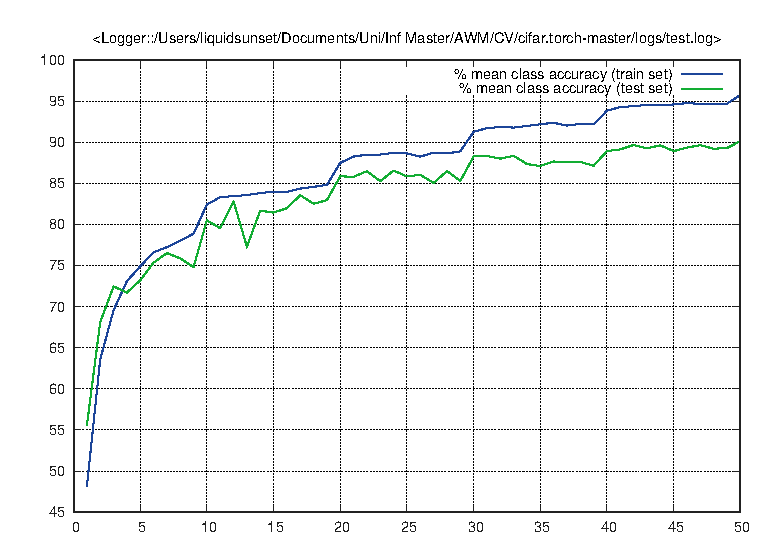
\includegraphics[scale=.7]{logs_nin/test.eps}
\caption{Network in Network 50 Epochs}
\label{fig:digraph}
\end{figure}

\begin{figure}[!htb]
\centering
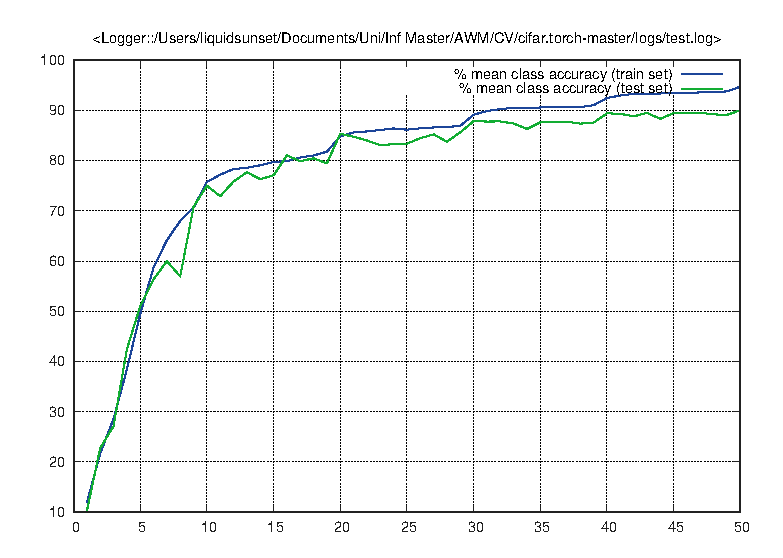
\includegraphics[scale=.7]{logs_vgg/test.eps}
\caption{VGG-Network 50 Epochs}
\label{fig:digraph}
\end{figure}

\begin{figure}[!htb]
\centering
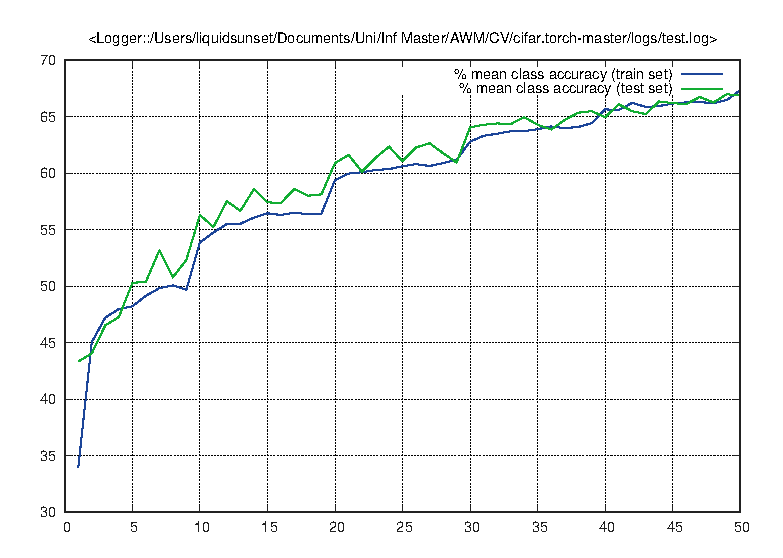
\includegraphics[scale=.7]{logs_assignment6/50_epochs/test.eps}
\caption{Assignment 6 Network 50 Epochs}
\label{fig:digraph}
\end{figure}

\begin{figure}[!htb]
\centering
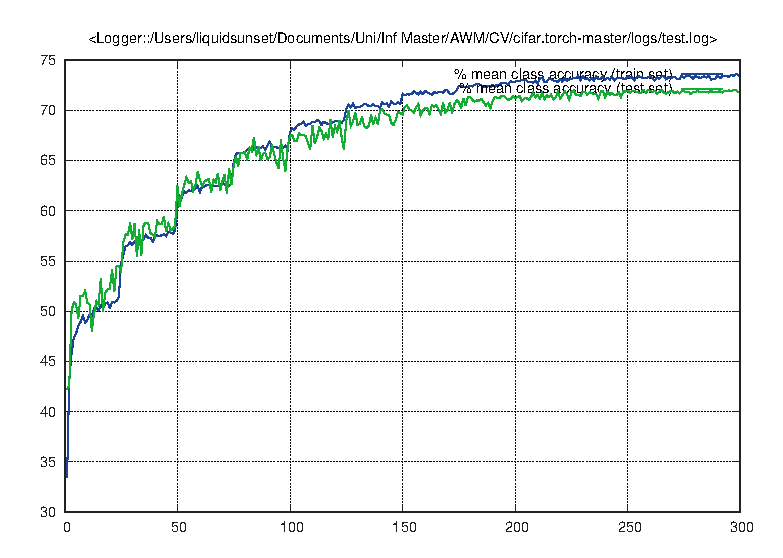
\includegraphics[scale=.7]{logs_assignment6/300_epochs/test.eps}
\caption{Assignment 6 Network 300 Epochs}
\label{fig:digraph}
\end{figure}

\FloatBarrier
\null\newpage

\begin{lstlisting}
--[[
Daniel Brand
Matr.-Nr.: 1023077
Computer Vision Assignment #6

This is a simple cnn for classifying the
cifar images (10 class problem)
--]]

-- import used packages
require 'nn'

-- define the network
local network = nn.Sequential()

--[[
applies 2D convolution within the input image over several input planes
number input planes: 3
number output planes: 12
Apply convolution with 5x5 (width x height) kernel
stepsize width dimension and height dimension: 1
additional zeros width and height-axis: 1
]]
network:add(nn.SpatialConvolution(3, 12, 5, 5, 1, 1, 1, 1))
--[[
applies 2D max-pooling
region-size: 2x2 (width x height)
step-size: 2x2 width dimension x height dimension
additional ceiling
]]
network:add(nn.SpatialMaxPooling(2, 2, 2, 2):ceil())

network:add(nn.Dropout())

network:add(nn.Tanh())

--[[
applies 2D convolution within the input image over several input planes
number input planes: 12
number output planes: 12
Apply convolution with 5x5 (width x height) kernel
stepsize width dimension and height dimension: 1
additional zeros width and height-axis: 1
]] 
network:add(nn.SpatialConvolution(12, 12, 5, 5, 1, 1, 1, 1))
--[[
applies 2D max-pooling
region-size: 2x2 (width x height)
step-size: 2x2 width dimension x height dimension
additional ceiling
]]
network:add(nn.SpatialMaxPooling(2, 2, 2, 2):ceil())
--[[
applies Tanh transfer function element-wise
]]
network:add(nn.Tanh())

--[[
applies 2D convolution within the input image over several input planes
number input planes: 12
number output planes: 14
Apply convolution with 5x5 (width x height) kernel
stepsize width dimension and height dimension: 1
additional zeros width and height-axis: 1
]] 
network:add(nn.SpatialConvolution(12, 24, 5, 5, 1, 1, 1, 1))
--[[
applies 2D max-pooling
region-size: 2x2 (width x height)
step-size: 2x2 width dimension x height dimension
additional ceiling
]]
network:add(nn.SpatialMaxPooling(2, 2, 2, 2):ceil())
--[[
applies Tanh transfer function element-wise
]]
network:add(nn.Tanh())

--[[
applies 2D convolution within the input image over several input planes
number input planes: 24
number output planes: 24
Apply convolution with 5x5 (width x height) kernel
stepsize width dimension and height dimension: 1
additional zeros width and height-axis: 1
]] 
network:add(nn.SpatialConvolution(24, 24, 5, 5, 1, 1, 1, 1))
--[[
applies 2D max-pooling
region-size: 2x2 (width x height)
step-size: 2x2 width dimension x height dimension
additional ceiling
]]
network:add(nn.SpatialMaxPooling(2, 2, 2, 2):ceil())
--[[
applies Tanh transfer function element-wise
]]
network:add(nn.Tanh())
--[[
reshaping the tensor to 1D
]]
network:add(nn.Reshape(24))
--[[
linear transformation
input size: 24
output size: 16
]]
network:add(nn.Linear(24, 16))
--[[
applies Tanh transfer function element-wise
]]
network:add(nn.Tanh())
--[[
linear transformation
input size: 24
output size: 10 -> 10 class classification problem 
]]
network:add(nn.Linear(16, 10))

-- initialization from MSR
local function MSRinit(net)
    local function init(name)
        for k, v in pairs(net:findModules(name)) do
            local n = v.kW * v.kH * v.nOutputPlane
            v.weight:normal(0, math.sqrt(2 / n))
            v.bias:zero()
        end
    end

    -- have to do for both backends
    init 'nn.SpatialConvolution'
end

MSRinit(network)

return network
\end{lstlisting}

\end{document}  